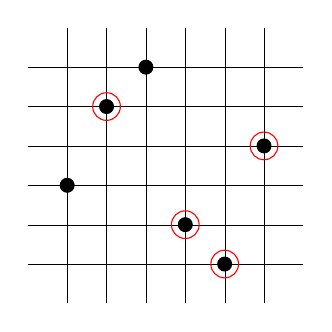
\begin{tikzpicture}[scale=.5,baseline=(current bounding box.center)]
    \foreach \x in {1,...,6} {
        \draw[ultra thin] (\x,0)--(\x,7); %vline
        \draw[ultra thin] (0,\x)--(7,\x); %hline
    }
    \draw[fill=black] (1,3) circle (5pt);
    \draw[fill=black] (2,5) circle (5pt);
    \draw[fill=black] (3,6) circle (5pt);
    \draw[fill=black] (4,2) circle (5pt);
    \draw[fill=black] (5,1) circle (5pt);
    \draw[fill=black] (6,4) circle (5pt);
    \draw[red] (2,5) circle (10pt);
    \draw[red] (4,2) circle (10pt);
    \draw[red] (5,1) circle (10pt);
    \draw[red] (6,4) circle (10pt);
\end{tikzpicture}